% intro.tex

\chapter{介绍}
\label{ch:intro}

长久以来,发明家们梦想着创造会思考的机器。这种愿望至少可以追溯到古希腊时代。神话
人物皮格马利翁,代达罗斯和赫菲斯托斯都可以被理解为传说中的发明家,而伽拉泰亚,塔
罗斯和潘多拉都可以被看作是人工生
命\citep{ovid2004metamorphoses,sparkes1996red,1997works}。

当可编程计算机最初被设想时~——~在它被建造的超过一百年前~——~人们就想知道它们是否可
能变得智能(Lovelace, 1842)。今天,\emph{\gls{ai} (AI)} 是一个茁壮成长的领域,有着
许多实际应用和活跃的研究课题。我们期待智能软件来自动化日常的劳动,理解语音或图像,
进行医学诊断和支持基础科学研究。

在\gls*{ai}早期,这个领域快速处理和解决一些问题,这些问题在脑力上对人类来说困难但
对计算机来说则相对直接~——~这些问题可以通过一份有条理的、数学规则的列表形式来描
述。\gls*{ai}的真正的挑战是解决那些容易被人执行,但是难于规范描述的任务~——~那些我
们凭直觉不假思索就能解决的问题,例如识别语音中的单词或者图像中的人脸。

这本书是关于这些更直观的问题的一个解决方案。这个解决方案是让计算机从经验中学习,
并以概念层次的形式理解这个世界,其中的每一个概念以和它相联系的更简单的概念形式定
义。通过从经验中收集知识,这种方法避免了需要人类操作者规范地去指定计算机需要的所
有知识。概念的层次结构允许计算机通过建立更简单的概念来学习复杂的概念。如果我们绘
制一个图,显示这些概念是如何建立在彼此之上的,这幅图会很深,有许多层。因为这个原
因,我们称这种人工智能的方法为\emph{\gls{dl}}。

许多早期的成功的人工智能发生在相对毫无新意和规范的环境中,并没有需要电脑有太多的
对世界的理解。例如,IBM 的深蓝对弈系统在 1997 年击败了世界冠军卡斯帕罗
夫\citep{Hsu2002}。国际象棋是一个很简单的世界,只包含 64 个位置和 32 个移动方式受
到严格限制的棋子。设计一个成功的国际象棋战略是一个巨大的成就,但是因为描述棋子的
集合和移动的困难性,这对计算机不算是挑战。象棋能够通过一个非常简短的完整规则的列
表来完整描述,很容易由程序员提前提供。

具有讽刺意味的是,对一个人类的来说最困难的脑力工作中那些抽象和规范的任务,对计算
机则是最简单的。计算机很早就能够击败即使是最优秀的人类国际象棋选手,但最近才能与
一般人的能力相匹配地识别物体或语音。一个人的日常生活需要大量的关于世界的知识。很
多这方面的知识是主观的和直观的,因此很难以一种规范的方式表达。计算机需要捕捉到相
同的知识,以便表现为一种智能的方式。人工智能中的一个关键的挑战是如何将这些非规范
的知识转化进计算机。

几个\gls*{ai}项目寻求用规范的语言来硬编码对于世界的理解。一台计算机可以自动使用逻
辑推理规则来对这些规范语言中的语句进行推理。这被称为人工智能
的\emph{\gls{knowledge-base}}\,方法。这些项目没有一个导致重大的成功。其中一个最著
名的项目是 Cyc\citep{Lenat-1989-book}。Cyc 是一个推理引擎和以一种称为 CycL 语言形
式的语句数据库。这些语句是由一个人类监督者输入的。这是一个笨拙的过程。人们费很大
劲来设计有条理的规则,这些规则具有足够的复杂性来准确描述这个世界。例如,Cyc 未能
理解一个关于一个名叫 Fred 的人在早晨刮脸的故事\citep{MachineChangedWorld}。它的推
理引擎检测到故事中前后矛盾的地方:它知道人类没有电子器件,但是因为 Fred 正好拿着
一个电子剃须刀,它坚信这个 ``正在刮脸的 Fred'' 包含有电子器件。于是它询问当 Fred
在刮脸时还是不是一个人类。

依赖于硬编码知识的系统面对的困难,表明 AI 系统需要获得它们自己知识的能力~——~通过
从原始数据中提取模式的能力。这个能力被称为\emph{\gls{ml}}。\gls*{ml}的引入允许计
算机处理涉及到真实世界的问题,并且做出显得主观的决定。一个简单的被称
为\emph{\gls{logistic-regression}}\,的\gls*{ml}算法能够确定是否建议剖腹
产 (Mor-Yosef et al., 1990)。另一个简单的被称为 \emph{naive Bayes} 的\gls*{ml}算
法,能够从垃圾邮件中区分出合理的邮件。

这些简单的\gls*{ml}算法的性能重度依赖给予它们的数据
的\emph{\gls{representations}}。例如,当\gls*{logistic-regression}被用在建议剖腹
产时,AI 系统不直接检查病人。相反,医生告诉这个系统一些相关信息,例如有没有子宫疤
痕。每段包含在病人描述中的信息被称为\emph{特征}。\gls*{logistic-regression}学习病
人的每个特征如何与不同的结果想关联。然而,它不能对任意方式定义的特征起作用。如果
给\gls*{logistic-regression}一幅病人的 MRI 扫描,而不是医生格式化后的报告,它无法
做出有用的预测。MRI 扫描中独特的像素和分娩中可能发生的并发症有负面的相关性。

这种对\gls*{representations}的依赖是一个普遍的现象,出现在整个计算机科学,甚至日
常生活中。在计算机科学中,诸如搜索一个数据的集合这样的操作,如果这个集合被很好地
结构化和智能地索引,那么这个搜索可以以指数级别加快处理,人们可以很容易地在阿拉伯
数字上执行算术运算,但在罗马数字做算术更为耗时。这是不足为奇的,
对\gls*{representations}的选择在\gls*{ml}算法的性能上有巨大的影响。一个简单的可视
化示例,参见图~\ref{fig:different_representations}。

\begin{figure}[h]
  \centering
  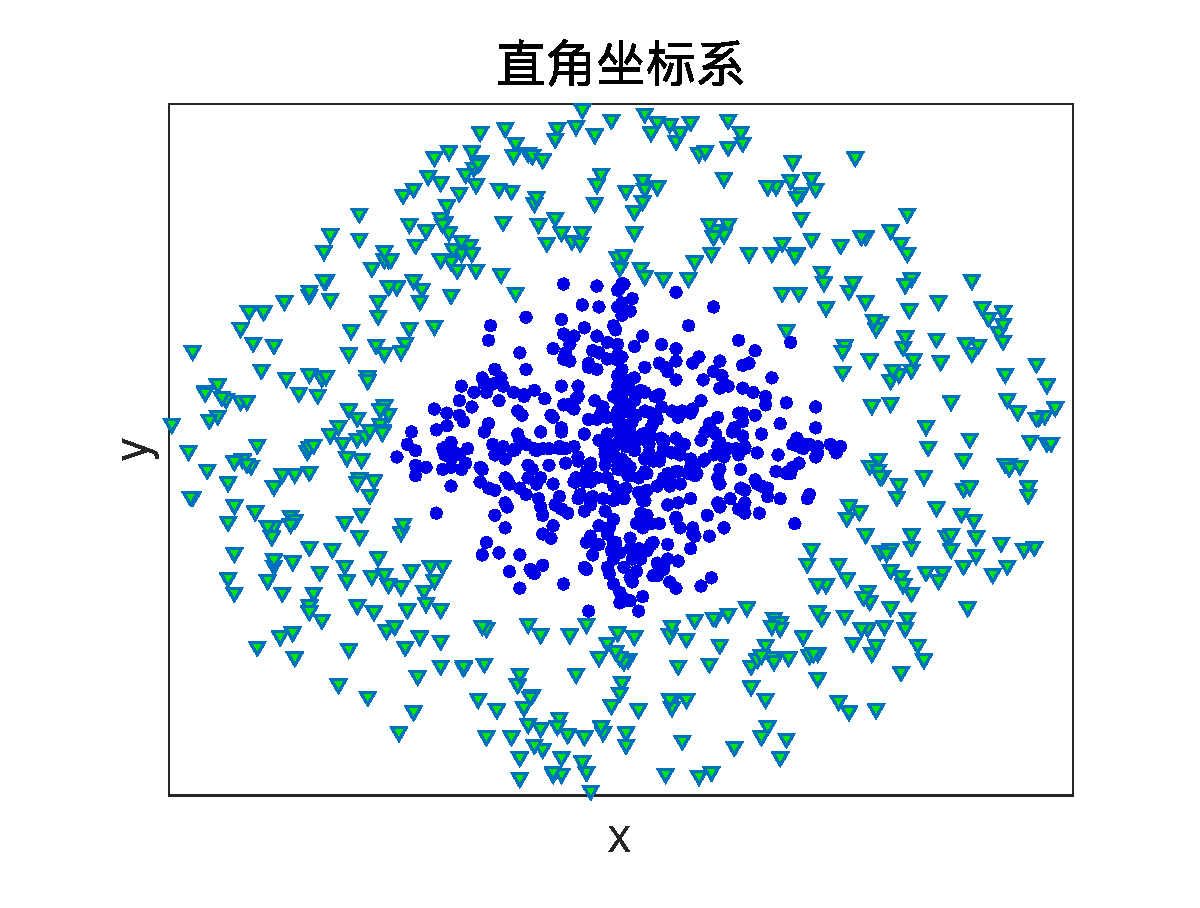
\includegraphics[width=0.45\textwidth]{cartesian_scatter}
  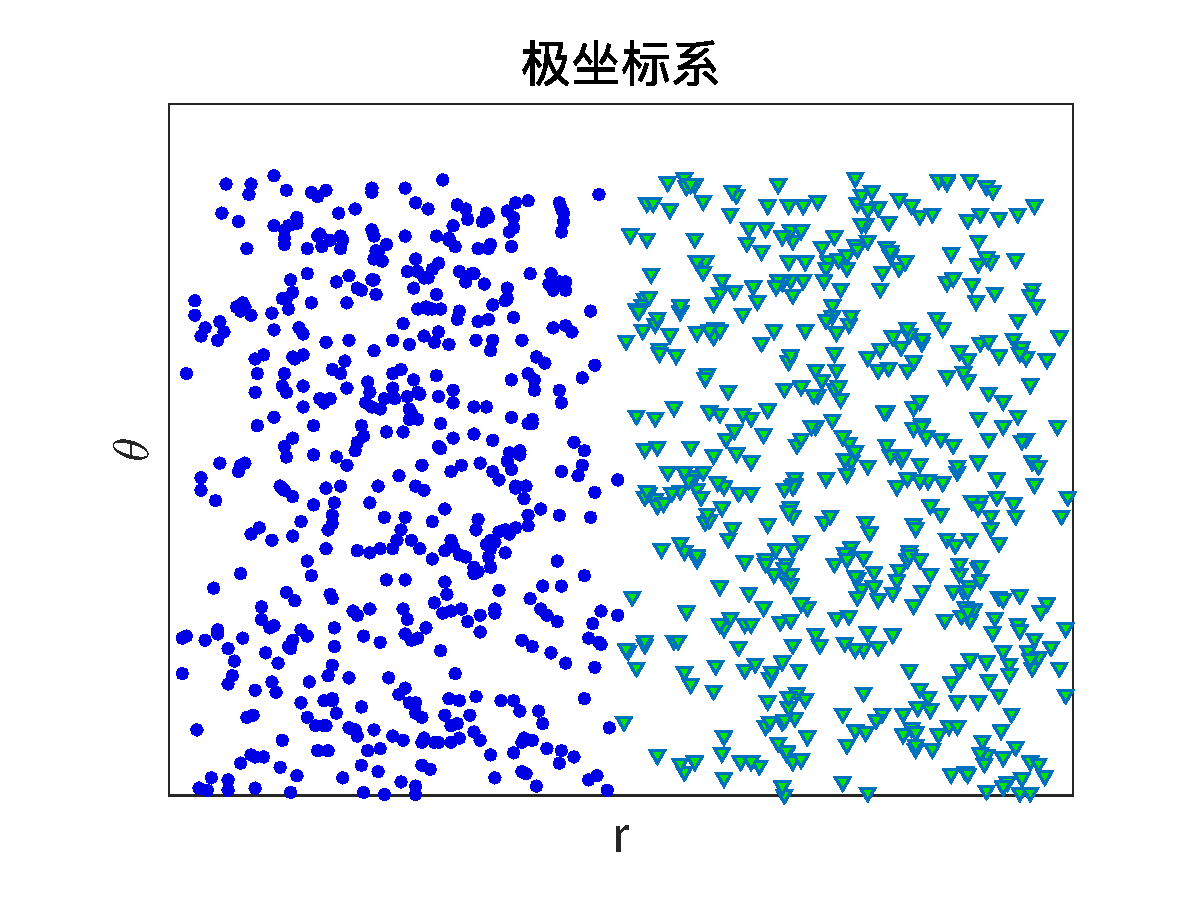
\includegraphics[width=0.45\textwidth]{polar_scatter}
  \caption{不同\gls*{representations}的例子:假设我们想要在一幅散点图中画一条线来
    区分两种数据。在左边的图中,我们使用笛卡尔坐标系描述一些数据,而这个任务是不
    可能的。在右边的图中,我们用极坐标描述一些数据,这个任务就变得很容易用一条竖
    线来解决。这个图由 David Warde-Farley 协助生
    成。\label{fig:different_representations}}
\end{figure}

这个问题的一个解决方法是使用\gls*{ml}来探索不只是从\gls*{representations}到输出的
映射,还有\gls*{representations}本身。这个方法被称为\emph{\gls{rep-learning}}。学
习过的\gls*{representations}往往会导致比手工设计的\gls*{representations}更好的性
能。它们还允许 AI 系统以最少的人为干预来快速地适应新的任务。一
个\gls*{rep-learning}算法可以在几分钟内为一个简单的任务发现一个很好的特征集,或者
对一个复杂的任务,需要几个小时到几个月。手动为一个复杂的任务设计特征需要大量的时
间和人力;它可能耗费整个研究社区几十年的时间。

一个\gls*{rep-learning}算法的典型例子是\emph{\gls{autoencoder}}。一
个\gls*{autoencoder}由一个\emph{\gls{encoder}}\,和一个\emph{\gls{decoder}}\,组
成,\gls*{encoder}将输入数据转换为不同形式的表征,\gls*{decoder}将新的表征转换回
原始格式。\gls*{autoencoder}被训练成当一个输入进
过\gls*{encoder}然后\gls*{decoder}时保存尽可能多的信息,但也被训练使得新的表征有
各种很好的特性。不同种类的\gls*{autoencoder}的目的是获得不同性质的特性。

当为了学习特征而设计特征或算法时,我们的目标通常是分离能解释被观察数据
的\emph{\gls{fov}}。在这种背景下,我们用单词``因子''来简单指不同的影响来源;因子
通常不由乘法组合。

\section{谁应该读这本书?}

\section{深度学习的历史趋势}



\subsection{不断增长的模型规模}
\label{subsec:increasing_model_sizes}
